%%%%%%%%%%%%%%%%%%%%%%%%%%%%%%%%%%%%%%%%%
%
% (c) 2019 by Jennifer Laaser
%
% This work is licensed under the Creative Commons Attribution-NonCommercial-ShareAlike 4.0 International License. To view a copy of this license, visit http://creativecommons.org/licenses/by-nc-sa/4.0/ or send a letter to Creative Commons, PO Box 1866, Mountain View, CA 94042, USA.
%
% The current source for these materials is accessible on Github: https://github.com/jlaaser/pogil-polymers
%
%%%%%%%%%%%%%%%%%%%%%%%%%%%%%%%%%%%%%%%%%

\renewcommand{\figpath}{content/polymphys/chain-confs/chain-elasticity/figs}
\renewcommand{\labelbase}{chain-elasticity}

\begin{activity}{Elasticity of Polymer Chains}

\begin{instructornotes}

	This activity introduces students to the concept of elasticity of polymer chains.
	
	After completing this activity, students will be able to:
			\begin{enumerate}
				\item \dots
			\end{enumerate}
	
			
	\subsection*{Activity summary:}
	\begin{itemize}
		\item \textbf{Activity type:} Learning Cycle
		\item \textbf{Content goals:} Basics of Chain Elasticity
		\item \textbf{Process goals:} %https://pogil.org/uploads/attachments/cj54b5yts006cklx4hh758htf-process-skills-official-pogil-list-2015-original.pdf
			\begin{itemize}
				\item \dots
			\end{itemize}
		\item \textbf{Duration:} approx. 60 minutes
		\item \textbf{Instructor preparation required:} 
			\begin{itemize}
				\item n/a
			\end{itemize}
		\item \textbf{Related textbook chapters:}
			\begin{itemize}
				\item \emph{Polymer Chemistry} (Hiemenz \& Lodge): Sections xx and yy
			\end{itemize}
	\end{itemize}

\end{instructornotes}

	%\textbf{Focus question:} Put a central question for the students to consider through this exercise here.

\begin{model}[Free Energy of Chain Stretching]
\label{model:delG}

	From basic thermodynamics, we know that the change in internal energy of a system during a process, $dU$, is
	\begin{equation*}
		dU = dq + dw
	\end{equation*}
	where $dq$ is the amount of heat transferred to the system and $dw$ is the amount of work done on the system.  We also know that the work done on a system is
	\begin{equation*}
		dw = f\,dL - P\,dV
	\end{equation*}
	where $f$ is the force acting on the material, $dL$ is the change in its length (the distance over which the force acts), $P$ is pressure, and $dV$ is change in volume.
	
	Using these relationships, it is possible to show that the change in Gibbs Free Energy is
	\begin{equation*}
		dG = f\,dL + V\,dP - S\,dT
	\end{equation*}
	where $S$ is entropy and $dT$ is change in temperature.

\end{model}


\begin{ctqs}

	\question Recall that for a function of three variables, $f(x,y,z)$, we can write
		\begin{equation*}
			df = \left(\frac{df}{dx}\right)_{y,z}dx + 
				\left(\frac{df}{dy}\right)_{x,z}dy +
				\left(\frac{df}{dz}\right)_{x,y}dz
		\end{equation*}
		Write an analogous expression for $dG$, assuming that G is a function of pressure ($P$), temperature ($T$), and the length $L$ of the material.
		
		\begin{solution}[1in]
		\end{solution}
		
	\question Compare your expression from the previous question to that given in Model 1.  What derivatives must each of the following values be equal to?
	
		\begin{enumerate}
			\item $f=$
				\begin{solution}[0.5in]
				\end{solution}
			\item $V=$
				\begin{solution}[0.5in]
				\end{solution}
			\item $S=$
				\begin{solution}[0.5in]
				\end{solution}
		\end{enumerate}
		
	\question Recall that $G = H - TS$, where $H$ is the enthalpy of the material.  
	
		Using this information, rewrite your expression for $f$ in terms of $\left(\frac{dH}{dL}\right)_{P,T}$ and $\left(\frac{dS}{dL}\right)_{P,T}$.  \emph{(Hint: you can assume that $T$ is constant.}
		
		\begin{solution}[1.5in]
		\end{solution}
		
		\label{\labelbase:ctq:fdSdL}
	
\end{ctqs}

\begin{infobox}
	
	For simplicity, we will consider only \emph{ideal elastomers}.
	
	An ideal elastomer is a material in which there is no significant change in the enthalpy with changes in length.
	
\end{infobox}

\begin{ctqs}

	\question Using this information, write an expression for $f$ only in terms of the temperature, $T$, entropy, $S$, and length of the sample, $L$.
		
		\begin{solution}[1in]
		\end{solution}
	
	\question What do you expect must need to be true about (1) the bond angles of the polymer, and (2) the surrounding environment in order for a polymer to behave as an ideal elastomer?  Explain your group's reasoning in 2-3 complete sentences.
		
		\begin{solution}[2in]
		\end{solution}

\end{ctqs}

\begin{model}[Stretching a Single Chain]
	To understand the force that it takes to stretch a polymer chain, we need to know something about how the entropy changes as we change the length of the polymer chain.
	
	Consider stretching a single polymer chain, as shown below:
	
	\vspace{6pt}
	\centerline{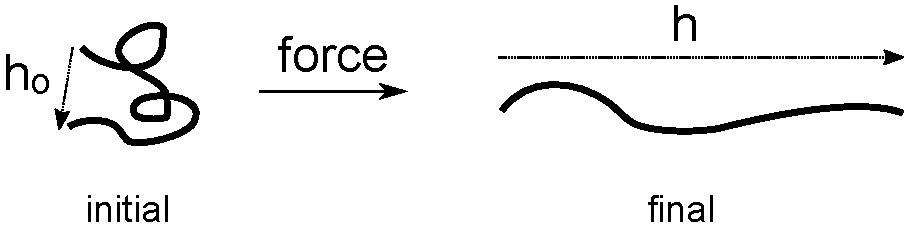
\includegraphics[width=0.55\textwidth]{\figpath/model2_chain-stretch.pdf}}
\end{model}

\begin{ctqs}
	\question Suppose that, in the initial state, the are $\Omega_i$ possible configurations of the chain that give end-to-end vector $\vec h_0$.  What is the entropy of this state?
	
		\emph{Hint: remember that $S = k\ln\Omega$.}
		
		\begin{solution}[0.5in]
		\end{solution}
	
	\question Suppose that in the final stretched state, there are $\Omega_f$ possible configurations of the chain that give end-to-end vector $\vec h$.  What is the entropy of this state?
		
		\begin{solution}[0.5in]
		\end{solution}
	
	\question Write an expression for the change in entropy that results from this stretching process, $\Delta S$, in terms of $\Omega_i$ and $\Omega_f$.
		
		\begin{solution}[1in]
		\end{solution}
	
\end{ctqs}

\begin{infobox}

	As you have learned, the conformations of flexible polymer chains can be described as a random walk.
	
	For a polymer chain with $N$ monomers with statistical segment length $b$, the number of conformations giving end-to-end vector $\vec h$ is
	\begin{equation*}
		\Omega(\vec h) = A e^{-3h^2/2Nb^2}
	\end{equation*}
	where $A$ is some proportionality constant and $h$ is the end-to-end distance.
	
\end{infobox}

\begin{ctqs}
	
	\question Using this information, rewrite your expression for $\Delta S$ in terms of the initial end-to-end distance $h_0$, the final end-to-end distance $h$, and any other necessary constants.
	
		\label{\labelbase:forcechain}
		
		\begin{solution}[2in]
		\end{solution}
	
	\question Since $h$ is essentially just the length of the chain, we can replace $L$ in the equation from CTQ \ref{\labelbase:ctq:fdSdL} with $h$ to obtain
		\begin{equation*}
			f = -T\left(\frac{d\Delta S}{dh}\right)
		\end{equation*}
		Using this expression, evaluate the force $f$ that it takes to stretch the chain to length $h$.
		
		\begin{solution}[2in]
		\end{solution}
		
	\question Compare your result to the following expression for the force required to extend a spring to length $x$:
		\begin{equation*}
			F = kx
		\end{equation*}
		(As you may recall from physics, this equation is \emph{Hooke's Law}.)
		
		\begin{enumerate}
			\item Which variable in CTQ \ref{\labelbase:forcechain} is analogous to the length of the spring, $x$?
		
				\begin{solution}[1in]
				\end{solution}
			
			\item Which collection of variables in CTQ \ref{\labelbase:forcechain} gives the spring constant, $k$?
		
				\begin{solution}[1in]
				\end{solution}
			
		\end{enumerate}
		
	\question Explain, in 2-3 complete sentences, why we often describe polymers as ``entropic springs.''
	
		\begin{solution}[2in]
		\end{solution}
	
\end{ctqs}
	
	
\begin{exercises}
	\exercise If you increase the temperature of a polymeric material, do you expect it to become stiffer (more difficult to stretch) or softer (easier to stretch)?  Explain your reasoning in 1-2 complete sentences.
\end{exercises}
	
\end{activity}